\documentclass[12pt,table,xcolor={dvipsnames}]{beamer}
%\usetheme{Pittsburgh}
\usecolortheme{seagull}
%\usepackage[utf8]{inputenc}
\usepackage{fontspec}
\usepackage[brazilian]{babel}
\usepackage{amsmath}
\usepackage{listings}
\usepackage{tikz}
\usetikzlibrary{calc,shapes.multipart,chains,arrows, positioning}
\usepackage{multirow}
\usepackage{amsfonts}
\usepackage{amssymb}
%\usepackage{lstlinebgrd}
\usepackage{graphicx}
\usepackage{wasysym}
\subtitle{Árvores}
\title{Estruturas de Dados}
%\setbeamercovered{transparent}
\setbeamertemplate{navigation symbols}{}
%\logo{\includegraphics[scale=0.015]{Brasao_UFSC.png}
\includegraphics[scale=0.2]{brasao_PPGCC.jpg}}
\institute{Departamento de Computação \\ Prof. Martín Vigil \\ Adaptado de prof. Jean Martina e Aldo Wangenheim}
\date{2020.1}
\subject{}
\usebackgroundtemplate{
\includegraphics[width=\paperwidth,
	height=\paperheight]{../reusable_images/fundo_UFSC.png}}
\begin{document}
	
	{
		\usebackgroundtemplate{
\includegraphics[width=\paperwidth,
			height=\paperheight]{../reusable_images/fundo_capa.png}}
		\begin{frame}
			\titlepage
			%
\includegraphics[scale=0.3]{../reusable_images/brasao_INE.png}
		\end{frame}
	}


\begin{frame}[fragile]{Introdução}
\lstset{language=C++,
          keywordstyle=\color{blue}\ttfamily,
          stringstyle=\color{red}\ttfamily,
          commentstyle=\color{OliveGreen}\ttfamily,
          breaklines=true,
          basicstyle=\ttfamily\footnotesize
          }
\begin{block}{Árvores}
são estruturas de dados que se caracterizam por uma organização hierárquica entre seus elementos. Essa organização permite a definição de algoritmos relativamente simples, recursivos e de eficiência bastante razoável.
\end{block}
\end{frame}

\begin{frame}[fragile]{Introdução}
\lstset{language=C++,
          keywordstyle=\color{blue}\ttfamily,
          stringstyle=\color{red}\ttfamily,
          commentstyle=\color{OliveGreen}\ttfamily,
          breaklines=true,
          basicstyle=\ttfamily\footnotesize
          }
\begin{itemize}
\item No cotidiano, diversas informações são organizadas de forma hierárquica;
\item Como exemplo, podem ser citados:
\begin{itemize}
\item  O organograma de uma empresa;
\item  A divisão de um livro em capítulos, seções, tópicos;
\item  A árvore genealógica de uma pessoa.
\end{itemize}
\end{itemize}
\end{frame}

\begin{frame}[fragile]{Introdução}
\lstset{language=C++,
          keywordstyle=\color{blue}\ttfamily,
          stringstyle=\color{red}\ttfamily,
          commentstyle=\color{OliveGreen}\ttfamily,
          breaklines=true,
          basicstyle=\ttfamily\footnotesize
          }
          \begin{center}
          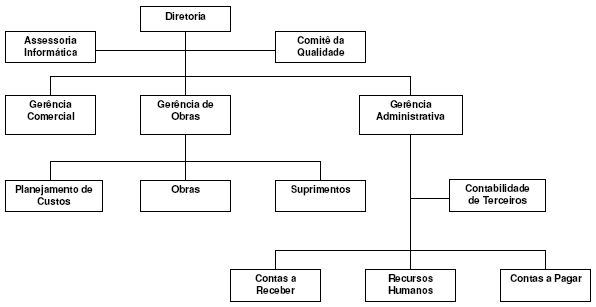
\includegraphics[scale=.5]{empresa.png} 
          \end{center}
\end{frame}

\begin{frame}[fragile]{Introdução}
\lstset{language=C++,
          keywordstyle=\color{blue}\ttfamily,
          stringstyle=\color{red}\ttfamily,
          commentstyle=\color{OliveGreen}\ttfamily,
          breaklines=true,
          basicstyle=\ttfamily\footnotesize
          }
\begin{itemize}
\item De um modo mais formal, podemos dizer que uma árvore é um conjunto finito de um ou mais nodos, nós ou vértices, tais que:
\begin{itemize}
\item  Existe um nodo denominado raiz da árvore;
\item  os demais nodos formam $n >= 0$ conjuntos disjuntos $c_1, c_2, ..., c_n$, sendo que cada um desses conjuntos também é uma árvore (denominada subárvore).
\end{itemize}
\end{itemize}
\end{frame}

\begin{frame}[fragile]{Representações}
\lstset{language=C++,
          keywordstyle=\color{blue}\ttfamily,
          stringstyle=\color{red}\ttfamily,
          commentstyle=\color{OliveGreen}\ttfamily,
          breaklines=true,
          basicstyle=\ttfamily\footnotesize
          }
          \begin{itemize}
		  \item Representação hierárquica
          \end{itemize}
          \begin{center}
          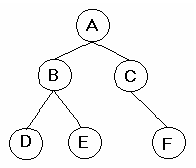
\includegraphics[scale=1]{tree.png} 
          \end{center}
\end{frame}
 
\begin{frame}[fragile]{Representações}
\lstset{language=C++,
          keywordstyle=\color{blue}\ttfamily,
          stringstyle=\color{red}\ttfamily,
          commentstyle=\color{OliveGreen}\ttfamily,
          breaklines=true,
          basicstyle=\ttfamily\footnotesize
          }
          \begin{itemize}
		  \item Representação por conjuntos (diagrama de inclusão)
          \end{itemize}
          \begin{center}
          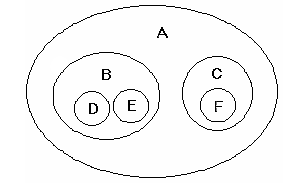
\includegraphics[scale=.95]{sets.png} 
          \end{center}
\end{frame} 

\begin{frame}[fragile]{Representações}
\lstset{language=C++,
          keywordstyle=\color{blue}\ttfamily,
          stringstyle=\color{red}\ttfamily,
          commentstyle=\color{OliveGreen}\ttfamily,
          breaklines=true,
          basicstyle=\ttfamily\footnotesize
          }
\begin{itemize}
\item Representação por expressão parentetizada (parênteses aninhados)
\begin{itemize}
\item  Cada conjunto de parênteses correspondentes contém um nodo e seus filhos. Se um nodo não tem filhos, ele é seguido por um par de parênteses sem conteúdo.
\end{itemize}
\end{itemize}
\begin{center}
 ( A ( \color{red} B ( \color{blue} D ( ) E ( ) \color{red}) \color{black} ) ( \color{red} C ( \color{blue}F ( ) \color{red} ) \color{black} ) )
\end{center}
\end{frame}

\begin{frame}[fragile]{Representações}
\lstset{language=C++,
          keywordstyle=\color{blue}\ttfamily,
          stringstyle=\color{red}\ttfamily,
          commentstyle=\color{OliveGreen}\ttfamily,
          breaklines=true,
          basicstyle=\ttfamily\footnotesize
          }
\begin{itemize}
\item Representação por expressão	não parentetizada
\begin{itemize}
\item  Cada nodo é seguido por um número que indica sua quantidade de filhos, e em seguida por cada um de seus filhos, representados do mesmo modo.
\end{itemize}
\end{itemize}
\begin{center}
\textbf{A 2 \color{red} B 2 \color{blue} D 0 E 0 \color{red} C 1 \color{blue} F 0} 
\end{center}
\end{frame}

\begin{frame}[fragile]{Representações}
\lstset{language=C++,
          keywordstyle=\color{blue}\ttfamily,
          stringstyle=\color{red}\ttfamily,
          commentstyle=\color{OliveGreen}\ttfamily,
          breaklines=true,
          basicstyle=\ttfamily\footnotesize
          }
\begin{itemize}
\item As duas primeiras representações permitem uma melhor visualização das árvores; 
\item As duas últimas, por sua vez, facilitam a persistência dos nodos das árvores (em arquivos, por exemplo), possibilitando assim a sua reconstituição.
\end{itemize}
\end{frame}

\begin{frame}[fragile]{Representações}
\lstset{language=C++,
          keywordstyle=\color{blue}\ttfamily,
          stringstyle=\color{red}\ttfamily,
          commentstyle=\color{OliveGreen}\ttfamily,
          breaklines=true,
          basicstyle=\ttfamily\footnotesize
          }
          \begin{itemize}
		  \item Como, por definição, os subconjuntos $c_1, c_2, ..., c_n$ são disjuntos, cada nodo pode ter apenas um pai. A representação a seguir, por exemplo, não corresponde a uma árvore.
          \end{itemize}
          \begin{center}
          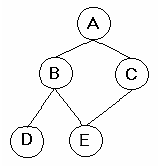
\includegraphics[scale=.75]{grafo.png} 
          \end{center}
\end{frame} 

\begin{frame}[fragile]{Definições}
\lstset{language=C++,
          keywordstyle=\color{blue}\ttfamily,
          stringstyle=\color{red}\ttfamily,
          commentstyle=\color{OliveGreen}\ttfamily,
          breaklines=true,
          basicstyle=\ttfamily\footnotesize
          }
          \begin{itemize}
		  \item A linha que liga dois nodos da árvore denomina-se aresta;
		  \item Existe um caminho entre dois nodos A e B da árvore, se a partir do nodo A é possível chegar ao nodo B percorrendo as arestas que ligam os nodos entre A e B;
		  \item Existe sempre um caminho entre a raiz e qualquer nodo da árvore.
          \end{itemize}
\end{frame} 

\begin{frame}[fragile]{Definições}
\lstset{language=C++,
          keywordstyle=\color{blue}\ttfamily,
          stringstyle=\color{red}\ttfamily,
          commentstyle=\color{OliveGreen}\ttfamily,
          breaklines=true,
          basicstyle=\ttfamily\footnotesize
          }
          \begin{itemize}
		  \item Se houver um caminho entre A e B, começando em A diz-se que A é um nodo ancestral de B e B é um nodo descendente de A
		  \item Se este caminho contiver uma única aresta, diz-se que A é o nodo pai de B e que B é um nodo filho de A; 
		  \item Dois nodos que são filhos do mesmo pai são denominados nodos irmãos;
		  \item Qualquer nodo, exceto a raiz, tem um único nodo pai.
          \end{itemize}
\end{frame} 

\begin{frame}[fragile]{Definições}
\lstset{language=C++,
          keywordstyle=\color{blue}\ttfamily,
          stringstyle=\color{red}\ttfamily,
          commentstyle=\color{OliveGreen}\ttfamily,
          breaklines=true,
          basicstyle=\ttfamily\footnotesize
          }
          \begin{itemize}
		  \item Se um nodo não possui nodos descendentes, ele é chamado de folha ou nodo terminal da árvore;
		  \item \textbf{Grau de um nodo}: é o número de nodos filhos do mesmo. Um nodo folha tem grau zero;
     	  \item \textbf{Nível de um nodo}: a raiz tem nível 0. Seus descendentes diretos têm nível 1, e assim por diante;
		  \item \textbf{Grau da árvore}: é igual ao grau do nodo de maior grau da árvore;
		  \item \textbf{Nível da árvore}: é igual ao nível do nodo de maior nível da árvore.
          \end{itemize}
\end{frame} 

\begin{frame}[fragile]{Exercício}
\lstset{language=C++,
          keywordstyle=\color{blue}\ttfamily,
          stringstyle=\color{red}\ttfamily,
          commentstyle=\color{OliveGreen}\ttfamily,
          breaklines=true,
          basicstyle=\ttfamily\footnotesize
          }
          \begin{center}
          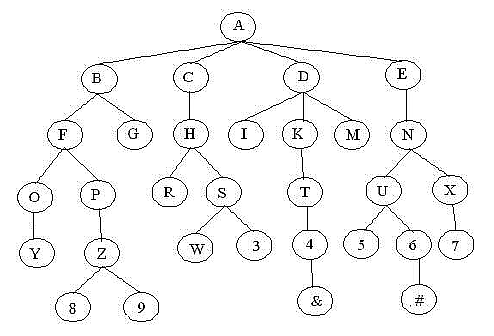
\includegraphics[scale=.55]{exercicio.png} 
          \end{center}
\end{frame} 



\begin{frame}[fragile]{Exercício}
\lstset{language=C++,
          keywordstyle=\color{blue}\ttfamily,
          stringstyle=\color{red}\ttfamily,
          commentstyle=\color{OliveGreen}\ttfamily,
          breaklines=true,
          basicstyle=\ttfamily\footnotesize
          }
          \begin{itemize}
          \item Qual é a raiz da árvore?
          \item Quais são os nodos terminais?
          \item Qual o grau da árvore?
          \item Qual o nível da árvore?
          \item Quais são os nodos descendentes do nodo D?
          \item Quais são os nodos ancestrais do nodo \#?
          \item Os nodos 4 e 5 são nodos irmãos?
          \item Há caminho entre os nodos C e S?
          \item Qual o nível do nodo 5?
          \item Qual o grau do nodo A?
          \end{itemize}
\end{frame} 

\begin{frame}[fragile]{Árvores Binárias}
\lstset{language=C++,
          keywordstyle=\color{blue}\ttfamily,
          stringstyle=\color{red}\ttfamily,
          commentstyle=\color{OliveGreen}\ttfamily,
          breaklines=true,
          basicstyle=\ttfamily\footnotesize
          }
          \begin{itemize}
          \item A inclusão de limitações estruturais define tipos específicos de árvores;
          \item Até agora, as árvores vistas possuíam nenhuma limitação quanto ao grau máximo de cada nodo;
          \item Uma árvore binária é uma árvore cujo grau máximo de cada nodo é 2. Essa limitação define uma nomenclatura específica: 
          \begin{itemize}
          \item As filhos de um nodo são classificados de acordo com sua posição relativa à raiz; 
          \item Assim, distinguem-se o filho da esquerda e o filho da direita e, consequentemente, a subárvore da esquerda e a subárvore da direita.         
          \end{itemize}
          \end{itemize}
\end{frame} 

\begin{frame}[fragile]{Árvores Binárias}
\lstset{language=C++,
          keywordstyle=\color{blue}\ttfamily,
          stringstyle=\color{red}\ttfamily,
          commentstyle=\color{OliveGreen}\ttfamily,
          breaklines=true,
          basicstyle=\ttfamily\footnotesize
          }
          \tikzset{
  treenode/.style = {align=center, inner sep=0pt, text centered,
    font=\sffamily},
  node_b/.style = {treenode, circle, white, font=\sffamily\bfseries, draw=black,
    fill=black, text width=1.5em},
  node_r/.style = {treenode, circle, red, draw=red, 
    text width=1.5em, very thick},
  node_s/.style = {treenode, circle, black, draw=black, 
    text width=1.5em, very thick},
  node_nil/.style = {treenode, rectangle, draw=black,
    minimum width=0.5em, minimum height=0.5em}
}
          \begin{itemize}
          \item Exemplo de árvore binária;
          \end{itemize}
          \begin{center}
          \begin{tikzpicture}[->,>=stealth',level/.style={sibling distance = 5cm/#1, level distance = 1.5cm}] 
\node [node_s] {A}
   child{ node [node_s] {B}
	   child{ node [node_s] {D}}
   	   child{ node [node_s] {E}}
   }
   child{ node [node_s] {C}
	   child{ node [node_s] {F} } 
	   child{ node [node_nil] {}}  
   }
; 
          \end{tikzpicture}
          \end{center}
\end{frame} 

\begin{frame}<0>[fragile]{Transformações}
\lstset{language=C++,
          keywordstyle=\color{blue}\ttfamily,
          stringstyle=\color{red}\ttfamily,
          commentstyle=\color{OliveGreen}\ttfamily,
          breaklines=true,
          basicstyle=\ttfamily\footnotesize
          }
          \begin{itemize}
          \item É possível transformar uma árvore n-ária em uma árvore binária através dos seguintes passos:
          	\begin{itemize}
          	\item A raiz da árvore (subárvore) será a raiz da árvore (subárvore) binária;
			\item O nodo filho mais à esquerda da raiz da árvore (subárvore) será o nodo filho à esquerda da raiz da árvore (subárvore) binária;
			\item Cada nodo irmão de B, da esquerda para a direita, será o nodo filho à direita do nodo irmão da esquerda, até que todos os nodos filhos da raiz da árvore (subárvore) já tenham sido incluídos na árvore binária em construção.
          	\end{itemize}

          \end{itemize}
\end{frame} 

\begin{frame}<0>[fragile]{Árvores Binárias}
\lstset{language=C++,
          keywordstyle=\color{blue}\ttfamily,
          stringstyle=\color{red}\ttfamily,
          commentstyle=\color{OliveGreen}\ttfamily,
          breaklines=true,
          basicstyle=\ttfamily\footnotesize
          }
          \tikzset{
  treenode/.style = {align=center, inner sep=0pt, text centered,
    font=\sffamily},
  node_b/.style = {treenode, circle, white, font=\sffamily\bfseries, draw=black,
    fill=black, text width=1.5em},
  node_r/.style = {treenode, circle, red, draw=red, 
    text width=1.5em, very thick},
  node_s/.style = {treenode, circle, black, draw=black, 
    text width=1.5em, very thick},
  node_nil/.style = {treenode, rectangle, draw=black,
    minimum width=0.5em, minimum height=0.5em}
}
          \begin{center}
          \begin{tikzpicture}[->,>=stealth',level/.style={sibling distance = 1.85cm/#1, level distance = 1.5cm}] 
\node [node_s] {A}
   child{ node [node_s] {B}
	   child{ node [node_s] {G}
	   	child{ node [node_s] {M}}
	   	child{ node [node_s] {N}}
	   }
   	   child{ node [node_s] {H}}
   	   child{ node [node_s] {I}}
   }
   child{ node [node_s] {C}}
   child{ node [node_s] {D}}
   child{ node [node_s] {E}
	   child{ node [node_s] {J} 
	   	child{ node [node_s] {O}}
	   } 
	   child{ node [node_s] {K}
	   	child{ node [node_s] {P}}		   
	   }  
   }
   child{ node [node_s] {F}}
   child{ node [node_s] {G}}
; 
          \end{tikzpicture}
          \end{center}
\end{frame} 

\begin{frame}<0>[fragile]{Árvores Binárias}
\lstset{language=C++,
          keywordstyle=\color{blue}\ttfamily,
          stringstyle=\color{red}\ttfamily,
          commentstyle=\color{OliveGreen}\ttfamily,
          breaklines=true,
          basicstyle=\ttfamily\footnotesize
          }
          \tikzset{
  treenode/.style = {align=center, inner sep=0pt, text centered,
    font=\sffamily},
  node_b/.style = {treenode, circle, white, font=\sffamily\bfseries, draw=black,
    fill=black, text width=1.5em},
  node_r/.style = {treenode, circle, red, draw=red, 
    text width=1.5em, very thick},
  node_s/.style = {treenode, circle, black, draw=black, 
    text width=1.5em, very thick},
  node_nil/.style = {treenode, rectangle, draw=black,
    minimum width=0.5em, minimum height=0.5em}
}
          \begin{center}
          \begin{tikzpicture}[->,>=stealth',level/.style={sibling distance = 8.5cm/#1, level distance = .8cm}] 
\node [node_s] {A}
   child{ node [node_s] {B}
	   child{ node [node_s] {G}
	   	child{ node [node_s] {M}
		   	child{ node [node_nil] {}}
		   	child{ node [node_s] {N}}
	   	}	   
	   	child{ node [node_s] {H}
		   	child{ node [node_nil] {}}
		   	child{ node [node_s] {I}}	   	
	   	}
	   }
	   child{ node [node_s] {C}
	   	child{ node [node_nil] {}}
	   	child{ node [node_s] {D}
		   	child{ node [node_nil] {}}
		   	child{ node [node_s] {E}
			   	child{ node [node_s] {J}
				   	child{ node [node_s] {O}}
				   	child{ node [node_s] {K}
					   	child{ node [node_nil] {}}
		   				child{ node [node_s] {P}}
				   	}	  			   	
			   	}
			   	child{ node [node_s] {F}
				   	child{ node [node_nil] {}}
				   	child{ node [node_s] {G}
					   	child{ node [node_nil] {}}
		   				child{ node [node_s] {L}}				   	
				   	}				   	
			   	}	  		   	
		   	}	     	
	   	}	   
	   }
   }
   child{ node [node_nil] {}}
; 
          \end{tikzpicture}
          \end{center}
\end{frame} 

\begin{frame}[fragile]{Modelagem: Nodo de uma árvore binária}
\lstset{language=C++,
          keywordstyle=\color{blue}\ttfamily,
          stringstyle=\color{red}\ttfamily,
          commentstyle=\color{OliveGreen}\ttfamily,
          breaklines=true,
          basicstyle=\ttfamily\footnotesize
          }
          \begin{itemize}
          \item Necessitamos:
          \begin{itemize}
          \item Um ponteiro para o filho localizado à esquerda;
          \item Um ponteiro para o filho localizado à direita;
          \item Um ponteiro \textbf{genérico} o dado que vamos armazenar.
          \end{itemize}
          \item Pseudo-código:
          \begin{lstlisting}
estrutura Nodo {
 Nodo *_filhoEsquerda;
 Nodo *_filhoDireita;
 T    *_dado;
};\end{lstlisting}
       	  \end{itemize}
\end{frame} 

\begin{frame}<0>[fragile]{Construção de uma árvore binária}
\lstset{language=C++,
          keywordstyle=\color{blue}\ttfamily,
          stringstyle=\color{red}\ttfamily,
          commentstyle=\color{OliveGreen}\ttfamily,
          breaklines=true,
          basicstyle=\ttfamily\footnotesize
          }
          \begin{itemize}
          \item Árvores como estruturas para organizar informações:
          \begin{itemize}
          \item Dados a serem inseridos em uma árvore são dados ordenáveis de alguma forma. Exemplo mais simples: números inteiros;
          \end{itemize}
          \item A árvore deverá possuir altura mínima:
          \begin{itemize}
          \item Caminhos médios de busca mínimos para uma mesma quantidade de dados.
          \end{itemize}
          \item Como fazer isso?
          \begin{itemize}
          \item garantir profundidades médias mínimas, preencher ao máximo cada nível antes de partir para o próximo e distribuir homogeneamente os nodos para a esquerda e direita.
          \end{itemize}
       	  \end{itemize}
\end{frame} 

\begin{frame}<0>[fragile]{Construção de uma árvore binária}
\lstset{language=C++,
          keywordstyle=\color{blue}\ttfamily,
          stringstyle=\color{red}\ttfamily,
          commentstyle=\color{OliveGreen}\ttfamily,
          breaklines=true,
          basicstyle=\ttfamily\footnotesize
          }
          \begin{itemize}
          \item Algoritmo:
          \begin{itemize}
          \item Use um nodo para a raiz;
          \item Gere a subárvore esquerda com nodosÀEsquerda = númeroDeNodos / 2 nodos, usando este mesmo procedimento;
          \item Gere a subárvore direita com nodosÀDireita = númeroDeNodos – nodosÀEsquerda - 1 nodos, usando este mesmo procedimento.
          \end{itemize}
       	  \end{itemize}
\end{frame}

\begin{frame}<0>[fragile]{Árvore Binária Balanceada}
\lstset{language=C++,
          keywordstyle=\color{blue}\ttfamily,
          stringstyle=\color{red}\ttfamily,
          commentstyle=\color{OliveGreen}\ttfamily,
          breaklines=true,
          basicstyle=\ttfamily\scriptsize
          }
          \begin{lstlisting}
tNodo* constróiÁrvore(inteiro númeroDeNodos)
 inteiro nodosÀEsquerda, nodosÀDireita;
 TipoInfo *info;
 tNodo *novoNodo;
 início
  se númeroDeNodos = 0 então
   retorna NULO;
  nodosÀEsquerda <- númeroDeNodos / 2;
  nodosÀDireita <- númeroDeNodos – nodosÀEsquerda – 1;
  aloque(info);
  ler(info);
  aloque(novoNodo);
  novoNodo->info <- info;
  novoNodo->filhoEsquerda <- constróiÁrvore(nodosÀEsquerda);
  novoNodo->filhoDireita <- constróiÁrvore(nodosÀDireita);
  retorna novoNodo;
 fim
		  \end{lstlisting}

\end{frame} 

\begin{frame}[fragile]{Percursos em Árvores Binárias}
\lstset{language=C++,
          keywordstyle=\color{blue}\ttfamily,
          stringstyle=\color{red}\ttfamily,
          commentstyle=\color{OliveGreen}\ttfamily,
          breaklines=true,
          basicstyle=\ttfamily\footnotesize
          }
          \begin{itemize}
          \item O percurso em árvores binárias corresponde ao caminhamento executado em listas: 
          \begin{itemize}
          \item Partimos de um nodo inicial (raiz) e visitamos todos os demais nodos em uma ordem previamente especificada;
          \end{itemize}
          \item Como exemplo, considere uma árvore binária utilizada para representar uma expressão (com as seguintes restrições):
          \begin{itemize}
          \item Cada operador representa uma bifurcação;
		  \item Seus dois operandos correspondentes são representados por suas subárvores.
          \end{itemize}
       	  \end{itemize}
\end{frame}

\begin{frame}[fragile]{Percursos em Árvores Binárias}
\lstset{language=C++,
          keywordstyle=\color{blue}\ttfamily,
          stringstyle=\color{red}\ttfamily,
          commentstyle=\color{OliveGreen}\ttfamily,
          breaklines=true,
          basicstyle=\ttfamily\footnotesize
          }
          \tikzset{
  treenode/.style = {align=center, inner sep=0pt, text centered,
    font=\sffamily},
  node_b/.style = {treenode, circle, white, font=\sffamily\bfseries, draw=black,
    fill=black, text width=1.5em},
  node_r/.style = {treenode, circle, red, draw=red, 
    text width=1.5em, very thick},
  node_s/.style = {treenode, circle, black, draw=black, 
    text width=1.5em, very thick},
  node_nil/.style = {treenode, rectangle, draw=black,
    minimum width=0.5em, minimum height=0.5em}
}
Expressão: (A + (B / X)) * (E - (C * P))
          \begin{center}
          \begin{tikzpicture}[->,>=stealth',level/.style={sibling distance = 5cm/#1, level distance = 1.5cm}] 
\node [node_s] {*}
   child{ node [node_s] {+}
	   child{ node [node_s] {A}}
   	   child{ node [node_s] {/}
   	   	   child{ node [node_s] {B}}
  	   	   child{ node [node_s] {X}}
   	   }
   }
   child{ node [node_s] {-}
   	child{ node [node_s] {E}}
   child{ node [node_s] {*}
    child{ node [node_s] {C}}   
    child{ node [node_s] {P}}   
   }
   }

; 
          \end{tikzpicture}
          \end{center}
\end{frame}

\begin{frame}[fragile]{Percursos em Árvores Binárias}
\lstset{language=C++,
          keywordstyle=\color{blue}\ttfamily,
          stringstyle=\color{red}\ttfamily,
          commentstyle=\color{OliveGreen}\ttfamily,
          breaklines=true,
          basicstyle=\ttfamily\footnotesize
          }
          \begin{itemize}
          \item Existem três ordens para se percorrer uma árvore binária que são consequência natural da estrutura da árvore, considerando filho à esquerda (e), filho à direita (a) e raiz (r):
          \begin{itemize}
          \item Preordem(r,e,d) – \textit{Preorder};
          \item Emordem(e,r,d) – \textit{Inorder};
          \item Pósordem(e,d,r) – \textit{Postorder}.
          \end{itemize}
       	  \end{itemize}
\end{frame}

\begin{frame}[fragile]{Percursos em Árvores Binárias}
\lstset{language=C++,
          keywordstyle=\color{blue}\ttfamily,
          stringstyle=\color{red}\ttfamily,
          commentstyle=\color{OliveGreen}\ttfamily,
          breaklines=true,
          basicstyle=\ttfamily\footnotesize
          }
          \begin{itemize}
          \item Essas ordens são definidas recursivamente (definição natural para uma árvore) e em função da raiz(r), da subárvore esquerda(e) e da subárvore direita(d):
          \begin{itemize}
          \item Preordem(r,e,d): visite a raiz ANTES das subárvores;
          \item Emordem(e,r,d): visite primeiro a subárvore ESQUERDA, depois a RAIZ e depois a subárvore DIREITA;
          \item Pósordem(e,d,r): visite a raiz DEPOIS das subárvores;
          \end{itemize}
          \item As subárvores são SEMPRE visitadas da esquerda para a direita.
       	  \end{itemize}
\end{frame}

\begin{frame}[fragile]{Percursos em Árvores Binárias}
\lstset{language=C++,
          keywordstyle=\color{blue}\ttfamily,
          stringstyle=\color{red}\ttfamily,
          commentstyle=\color{OliveGreen}\ttfamily,
          breaklines=true,
          basicstyle=\ttfamily\footnotesize
          }
          \begin{itemize}
          \item Se percorrermos a árvore anterior usando as ordens definidas, teremos as seguintes seqüências:
          \begin{itemize}
          \item Preordem (notação prefixada) : * + A	/ B X - E * C P
          \item Emordem (notação infixada) : A + B / X * E - C * P
          \item Pósordem (notação posfixada) : A B X / + * E C P - *
          \end{itemize}
       	  \end{itemize}
         
\tikzset{
	treenode/.style = {align=center, inner sep=0pt, text centered,
		font=\sffamily},
	node_b/.style = {treenode, circle, white, font=\sffamily\bfseries, draw=black,
		fill=black, text width=1.5em},
	node_r/.style = {treenode, circle, red, draw=red, 
		text width=1.5em, very thick},
	node_s/.style = {treenode, circle, black, draw=black, 
		text width=1.5em, very thick},
	node_nil/.style = {treenode, rectangle, draw=black,
		minimum width=0.5em, minimum height=0.5em}
}
\begin{center}
	\resizebox{!}{4cm}{\begin{tikzpicture}[->,>=stealth',level/.style={sibling distance = 5cm/#1, level distance = 1.5cm}] 
	\node [node_s] {*}
	child{ node [node_s] {+}
		child{ node [node_s] {A}}
		child{ node [node_s] {/}
			child{ node [node_s] {B}}
			child{ node [node_s] {X}}
		}
	}
	child{ node [node_s] {-}
		child{ node [node_s] {E}}
		child{ node [node_s] {*}
			child{ node [node_s] {C}}   
			child{ node [node_s] {P}}   
		}
	}
	
	; 
	\end{tikzpicture}}
\end{center}

         
\end{frame}

\begin{frame}[fragile]{Percurso em Preordem}
\lstset{language=C++,
          keywordstyle=\color{blue}\ttfamily,
          stringstyle=\color{red}\ttfamily,
          commentstyle=\color{OliveGreen}\ttfamily,
          breaklines=true,
          basicstyle=\ttfamily\footnotesize
          }
          \begin{lstlisting}
Lista* Preordem(Nodo *raiz)
 início
  ListaEncadeada* lista = iniciaListaEncadeada();
  se raiz != NULO então
   adicionaNoFim(lista, raiz->_dado);
   Preordem(raiz->_filhoEsquerda);
   Preordem(raiz->_filhoDireita);
  fim se
 fim
 \end{lstlisting}
\end{frame} 

\begin{frame}[fragile]{Percurso em Emordem}
\lstset{language=C++,
          keywordstyle=\color{blue}\ttfamily,
          stringstyle=\color{red}\ttfamily,
          commentstyle=\color{OliveGreen}\ttfamily,
          breaklines=true,
          basicstyle=\ttfamily\footnotesize
          }
          \begin{lstlisting}
Lista* EmOrdem(Nodo *raiz)
 início
  ListaEncadeada* lista = iniciaListaEncadeada();
  se raiz != NULO então
   EmOrdem(raiz->_filhoEsquerda);
   adicionaNoFim(lista, raiz->_dado);
   EmOrdem(raiz->_filhoDireita);
  fim se
 fim
\end{lstlisting}
\end{frame} 

\begin{frame}[fragile]{Percurso em Posordem}
\lstset{language=C++,
          keywordstyle=\color{blue}\ttfamily,
          stringstyle=\color{red}\ttfamily,
          commentstyle=\color{OliveGreen}\ttfamily,
          breaklines=true,
          basicstyle=\ttfamily\footnotesize
          }
          \begin{lstlisting}
Lista PosOrdem(tNodo *raiz)
 início
  ListaEncadeada* lista = iniciaListaEncadeada();
  se raiz != NULO então
   PosOrdem(raiz->_filhoEsquerda);
   PosOrdem(raiz->_filhoDireita);
   adicionaNoFim(raiz->_dado);
  fim se
 fim
 \end{lstlisting}
\end{frame} 

\begin{frame}[fragile]{Árvores Binárias de Busca}
\lstset{language=C++,
          keywordstyle=\color{blue}\ttfamily,
          stringstyle=\color{red}\ttfamily,
          commentstyle=\color{OliveGreen}\ttfamily,
          breaklines=true,
          basicstyle=\ttfamily\footnotesize
          }
          \begin{itemize}
          \item Árvores (binárias) são muito utilizadas para se representar um grande conjunto de dados onde se deseja encontrar um elemento de acordo com a sua chave.
          \item Definição - Árvore Binária de Busca (Niklaus Wirth):
          \begin{itemize}
          \item “Uma árvore que se encontra organizada de tal forma que, para cada nodo $t_i$, todas as chaves (\_dado) da subárvore à esquerda de $t_i$ são menores que $t_i$ e à direita são maiores (ou iguais) que $t_i$";
          \end{itemize}
          \item Termo em Inglês: Search Tree.
       	  \end{itemize}
\end{frame}

\begin{frame}[fragile]{Características de Árvores Binárias de Busca}
\lstset{language=C++,
          keywordstyle=\color{blue}\ttfamily,
          stringstyle=\color{red}\ttfamily,
          commentstyle=\color{OliveGreen}\ttfamily,
          breaklines=true,
          basicstyle=\ttfamily\footnotesize
          }
          \begin{itemize}
          \item Em uma árvore binária de busca é possível encontrar-se qualquer chave existente descendo-se pela árvore:
          \begin{itemize}
          \item Sempre à esquerda toda vez que a chave procurada for menor do que a chave do nodo visitado;
          \item Sempre à direita toda vez que for maior ou igual;
          \end{itemize}
          \item A escolha da direção de busca só depende da chave que se procura e da chave que o nodo atual possui.
       	  \end{itemize}
\end{frame}

\begin{frame}[fragile]{Características de Árvores Binárias de Busca}
\lstset{language=C++,
          keywordstyle=\color{blue}\ttfamily,
          stringstyle=\color{red}\ttfamily,
          commentstyle=\color{OliveGreen}\ttfamily,
          breaklines=true,
          basicstyle=\ttfamily\footnotesize
          }
          \begin{itemize}
          \item A busca de um elemento em uma árvore balanceada com n elementos toma tempo médio < log(n), sendo a busca então O(log n);
          \item Graças à estrutura de árvore a busca poderá ser feita com apenas log(n) comparações de elementos.
       	  \end{itemize}
\end{frame}

\begin{frame}[fragile]{Exemplo de árvore binária de busca}
\setbeamercovered{invisible}
\begin{center}
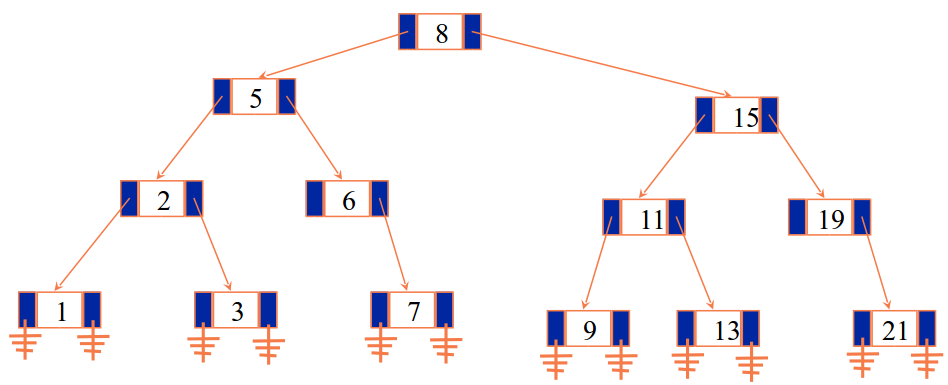
\includegraphics[scale=.3]{arv1.png} 
\end{center}
\end{frame}

\begin{frame}[fragile]{Algoritmo de Busca}
\lstset{language=C++,
          keywordstyle=\color{blue}\ttfamily,
          stringstyle=\color{red}\ttfamily,
          commentstyle=\color{OliveGreen}\ttfamily,
          breaklines=true,
          basicstyle=\ttfamily\footnotesize
          }
          \begin{lstlisting}
Nodo* busca (T dado, Nodo* raiz)
 início
  enquanto(raiz != NULO E raiz->_dado != dado) faça
   // Esquerda ou direita.
   se (raiz->_dado < dado) então
    raiz <- raiz->filhoDireita
   senão
    raiz <- raiz->filhoEsquerda;
   fim se
  fim enquanto
  retorne raiz;
 fim
 \end{lstlisting}
\end{frame} 

\begin{frame}[fragile]{Exemplo}
\setbeamercovered{invisible}
Inserção de um elemento com chave = 14
\begin{center}
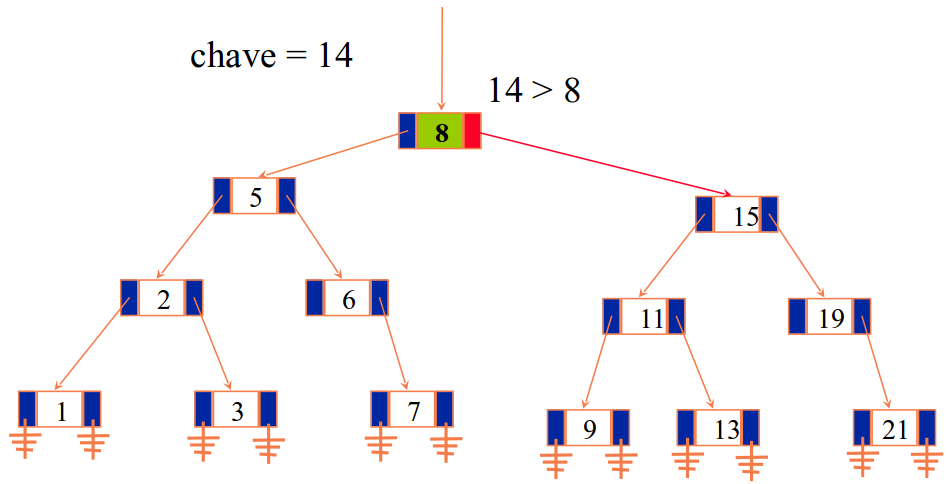
\includegraphics[scale=.3]{arv2.png} 
\end{center}
\end{frame}

\begin{frame}[fragile]{Exemplo}
\setbeamercovered{invisible}
Inserção de um elemento com chave = 14
\begin{center}
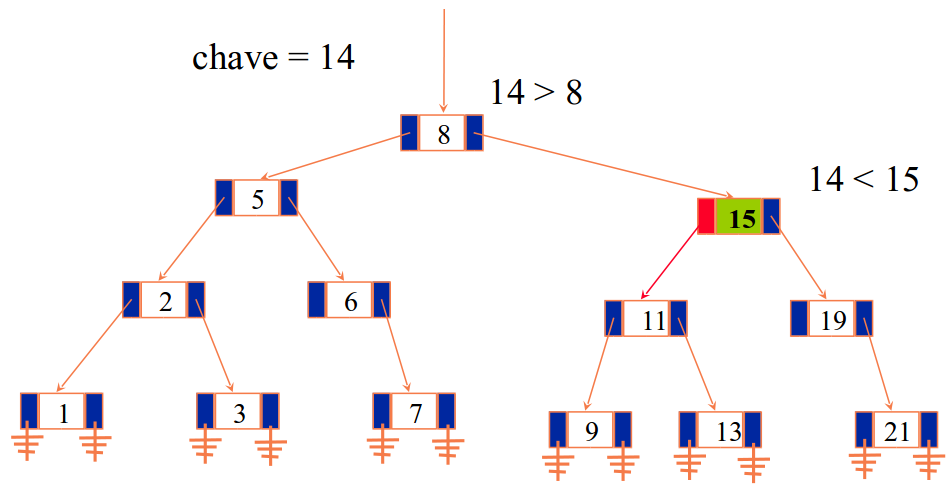
\includegraphics[scale=.3]{arv3.png} 
\end{center}
\end{frame}

\begin{frame}[fragile]{Exemplo}
\setbeamercovered{invisible}
Inserção de um elemento com chave = 14
\begin{center}
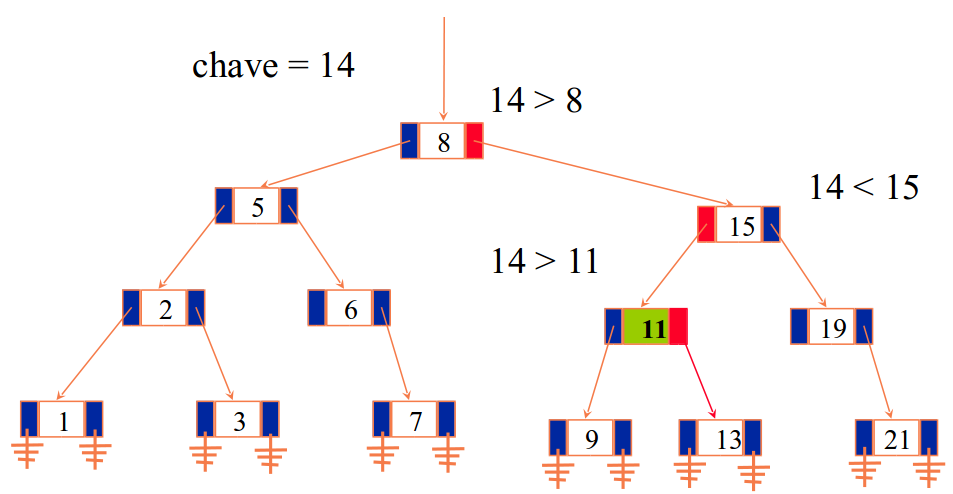
\includegraphics[scale=.3]{arv4.png} 
\end{center}
\end{frame}

\begin{frame}[fragile]{Exemplo}
\setbeamercovered{invisible}
Inserção de um elemento com chave = 14
\begin{center}
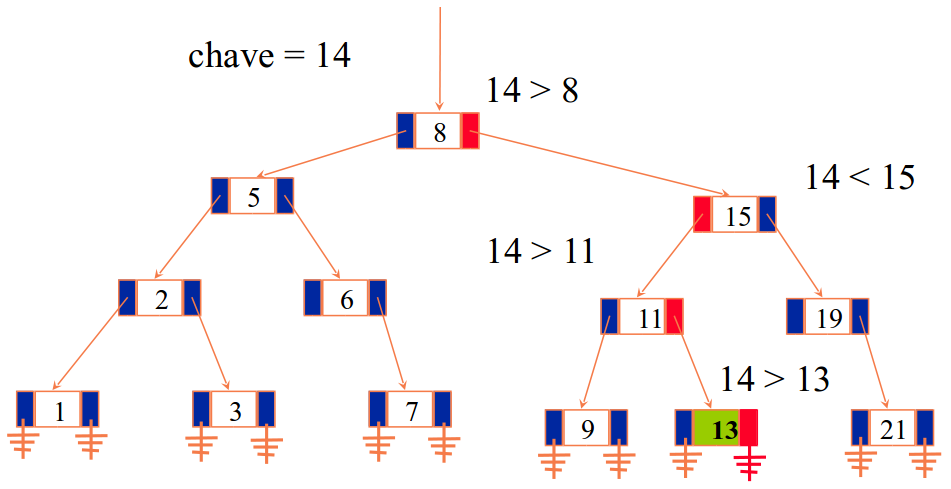
\includegraphics[scale=.3]{arv5.png} 
\end{center}
\end{frame}

\begin{frame}[fragile]{Exemplo}
\setbeamercovered{invisible}
Inserção de um elemento com chave = 14
\begin{center}
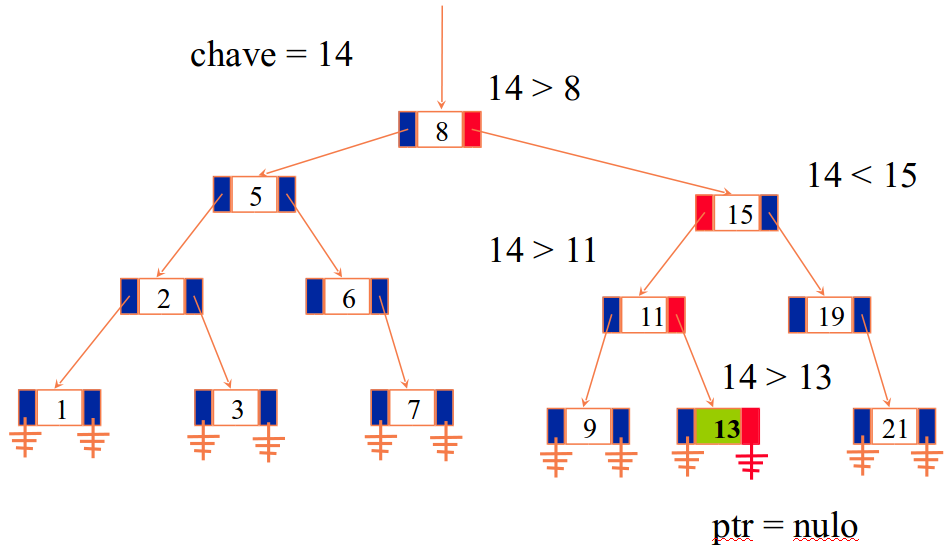
\includegraphics[scale=.3]{arv6.png} 
\end{center}
\end{frame}

\begin{frame}[fragile]{Exemplo}
\setbeamercovered{invisible}
Inserção de um elemento com chave = 14
\begin{center}
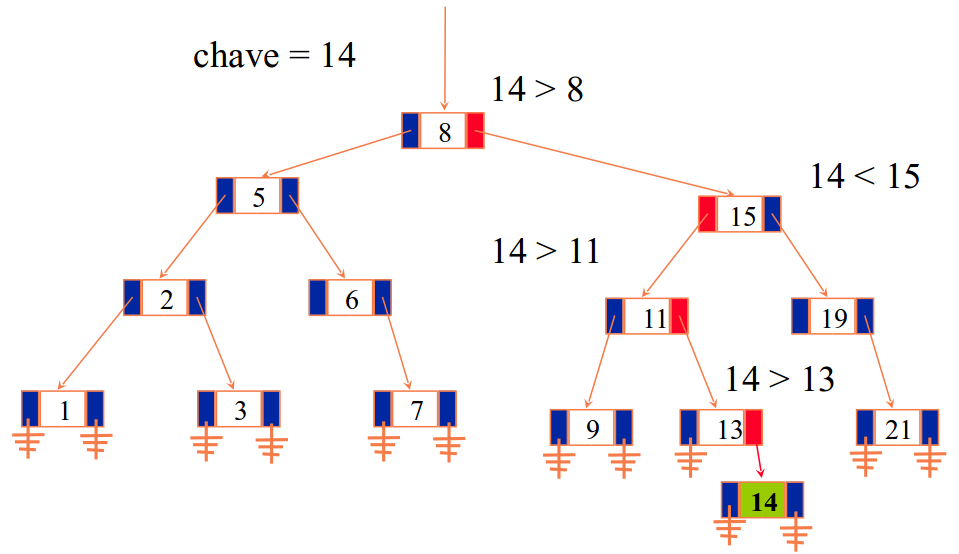
\includegraphics[scale=.3]{arv7.png} 
\end{center}
\end{frame}

\begin{frame}[fragile]{Algoritmo de Inserção}
\lstset{language=C++,
          keywordstyle=\color{blue}\ttfamily,
          stringstyle=\color{red}\ttfamily,
          commentstyle=\color{OliveGreen}\ttfamily,
          breaklines=true,
          basicstyle=\ttfamily\scriptsize
          }
          \begin{lstlisting}
void inserir(Nodo* raiz, T* dado)
 início
  se (dado < raiz->_dado) então
  // Inserção à esquerda.
   se (raiz->_filhoEsquerda = NULO) então
    Nodo* oNovo <- aloque(Nodo); oNovo->_dado <- dado;
    oNovo->filhoEsquerda <- NULO; oNovo->filhoDireita <- NULO;
    raiz->filhoÀEsquerda <- oNovo;
   senão
    inserir(raiz->_filhoEsquerda, dado);
   fim se
   senão
    // Inserção à direita.
   se (raiz->filhoDireita = NULO) então
    Nodo* oNovo <- aloque(Nodo); oNovo->_dado <- dado;
    oNovo->filhoEsquerda <- NULO; oNovo->filhoDireita <- NULO;
    raiz->filhoÀDireita <- oNovo;
   senão
    inserir(raiz->filhoDireita, dado);
   fim se
  fim se  
 fim
 \end{lstlisting}
\end{frame} 

\begin{frame}[fragile]{Algoritmo de Deleção}
\lstset{language=C++,
          keywordstyle=\color{blue}\ttfamily,
          stringstyle=\color{red}\ttfamily,
          commentstyle=\color{OliveGreen}\ttfamily,
          breaklines=true,
          basicstyle=\ttfamily\footnotesize
          }
          \begin{itemize}
          \item A deleção é mais complexa do que a inserção;
		  \item A razão básica é que a característica organizacional da árvore não deve ser quebrada:
		  \begin{itemize}
		  \item A subárvore da direita de um nodo não deve possuir chaves menores do que o pai do nodo eliminado;
		  \item A subárvore da esquerda de um nodo não deve possuir chaves maiores do que o pai do nodo eliminado.
		  \end{itemize}
		  \item Para garantir isso, o algoritmo de deleção deve remanejar os nodos.
       	  \end{itemize}
\end{frame}

\begin{frame}[fragile]{Exemplo}
\setbeamercovered{invisible}
Deleção do nodo com chave = 15
\begin{center}
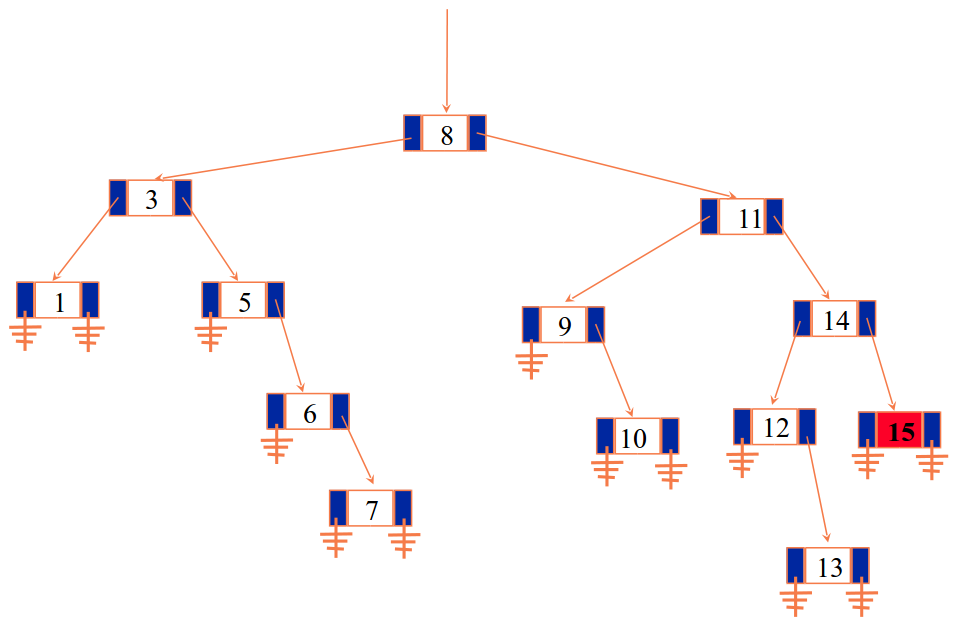
\includegraphics[scale=.3]{arv8.png} 
\end{center}
\end{frame}

\begin{frame}[fragile]{Exemplo}
\setbeamercovered{invisible}
Deleção do nodo com chave = 15
\begin{center}
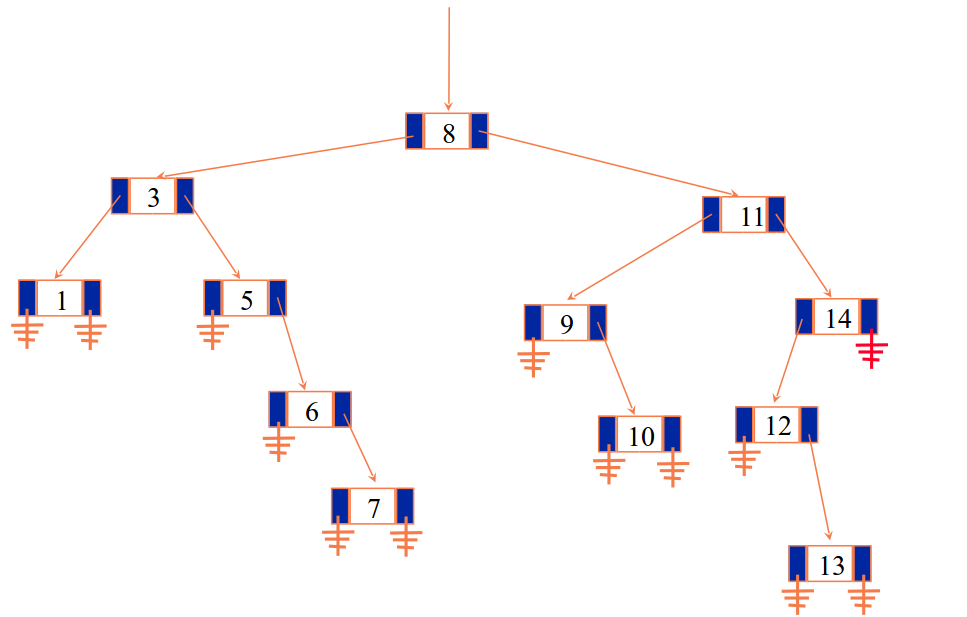
\includegraphics[scale=.3]{arv9.png} 
\end{center}
\end{frame}

\begin{frame}[fragile]{Deleção em uma Arvore de Busca Binária}
\lstset{language=C++,
          keywordstyle=\color{blue}\ttfamily,
          stringstyle=\color{red}\ttfamily,
          commentstyle=\color{OliveGreen}\ttfamily,
          breaklines=true,
          basicstyle=\ttfamily\footnotesize
          }
          \begin{itemize}
          \item Se o nodo possuir somente uma subárvore filha:
		  \begin{itemize}
		  \item Podemos simplesmente mover esta subárvore toda para cima;
		  \item O único sucessor do nodo a ser excluído será um dos sucessores diretos do pai do nodo a ser eliminado;
		  \item Se o nodo a ser excluído é filho esquerdo de seu pai, o seu filho será o novo filho esquerdo deste e vice-versa.
		  \end{itemize}
       	  \end{itemize}
\end{frame}

\begin{frame}[fragile]{Exemplo}
\setbeamercovered{invisible}
Deleção do nodo com chave = 5
\begin{center}
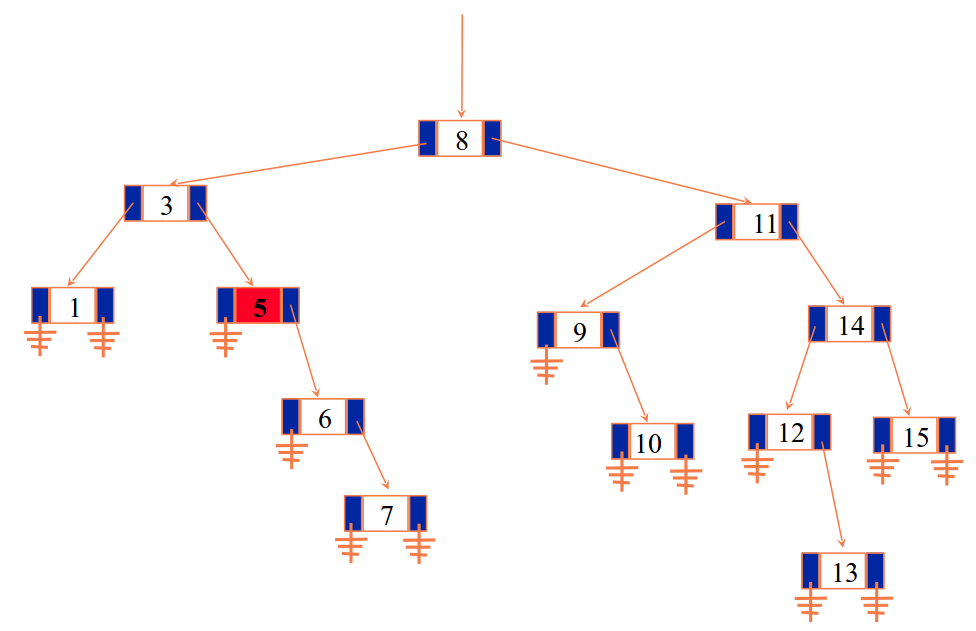
\includegraphics[scale=.3]{arv10.png} 
\end{center}
\end{frame}

\begin{frame}[fragile]{Exemplo}
\setbeamercovered{invisible}
Deleção do nodo com chave = 5
\begin{center}
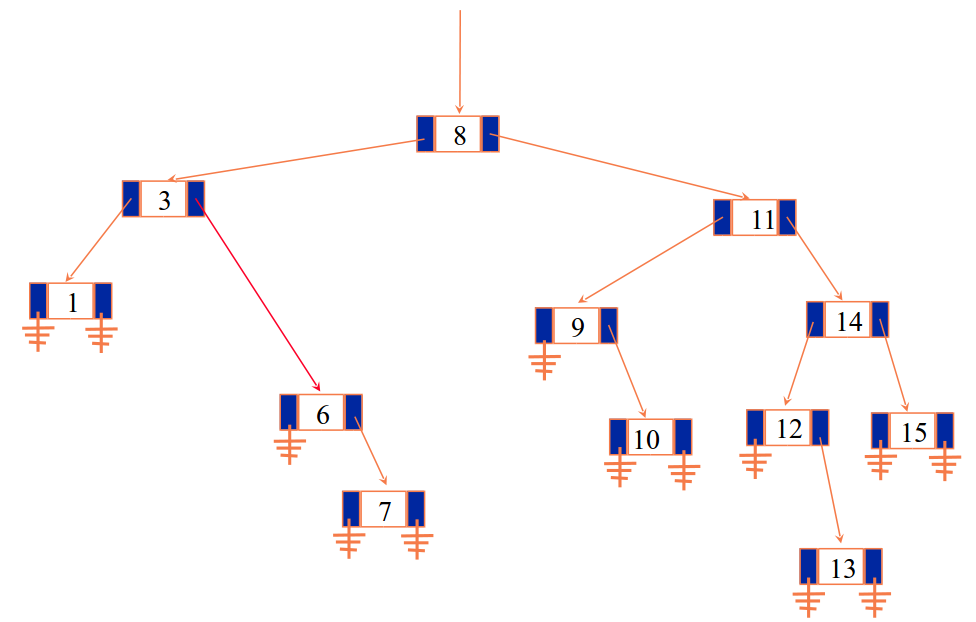
\includegraphics[scale=.3]{arv11.png} 
\end{center}
\end{frame}

\begin{frame}[fragile]{Exemplo}
\setbeamercovered{invisible}
Deleção do nodo com chave = 5
\begin{center}
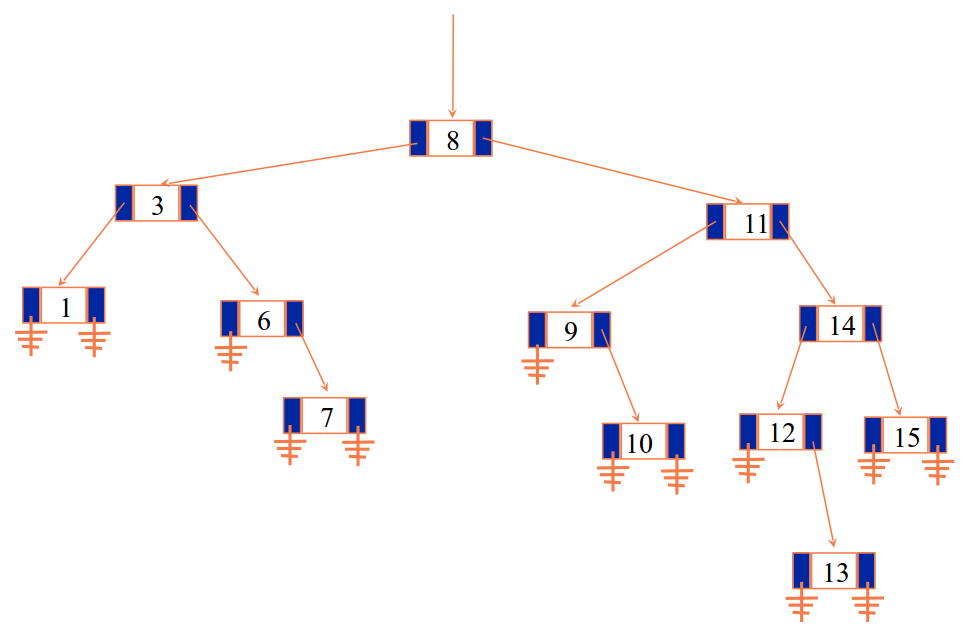
\includegraphics[scale=.3]{arv12.png} 
\end{center}
\end{frame}

\begin{frame}[fragile]{Deleção em uma Arvore de Busca Binária}
\lstset{language=C++,
          keywordstyle=\color{blue}\ttfamily,
          stringstyle=\color{red}\ttfamily,
          commentstyle=\color{OliveGreen}\ttfamily,
          breaklines=true,
          basicstyle=\ttfamily\footnotesize
          }
          \begin{itemize}
          \item Se o nodo possuir duas subárvores filhas:
		  \begin{itemize}
		  \item Se o filho à direita não possui subárvore esquerda, é ele quem ocupa o seu lugar;
		  \item Se possuir uma subárvore esquerda, a raiz desta será movida para cima e assim por diante;
		  \item A estratégia geral (Mark Allen Weiss) é sempre substituir a chave retirada pela menor chave da subárvore direita.
		  \end{itemize}
       	  \end{itemize}
\end{frame}

\begin{frame}[fragile]{Exemplo}
\setbeamercovered{invisible}
Deleção do nodo com chave = 11
\begin{center}
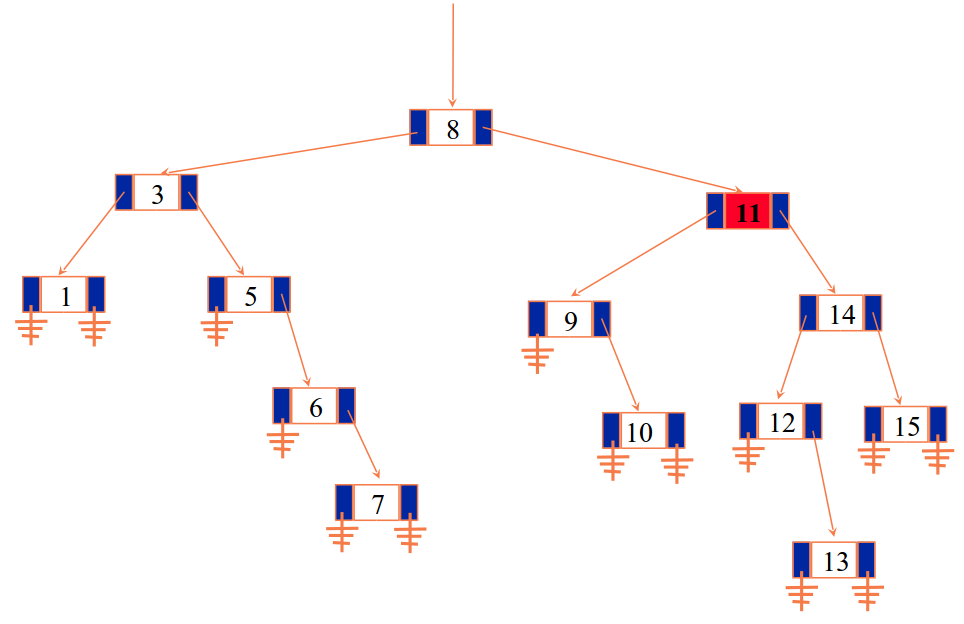
\includegraphics[scale=.3]{arv13.png} 
\end{center}
\end{frame}

\begin{frame}[fragile]{Exemplo}
\setbeamercovered{invisible}
Deleção do nodo com chave = 5
\begin{center}
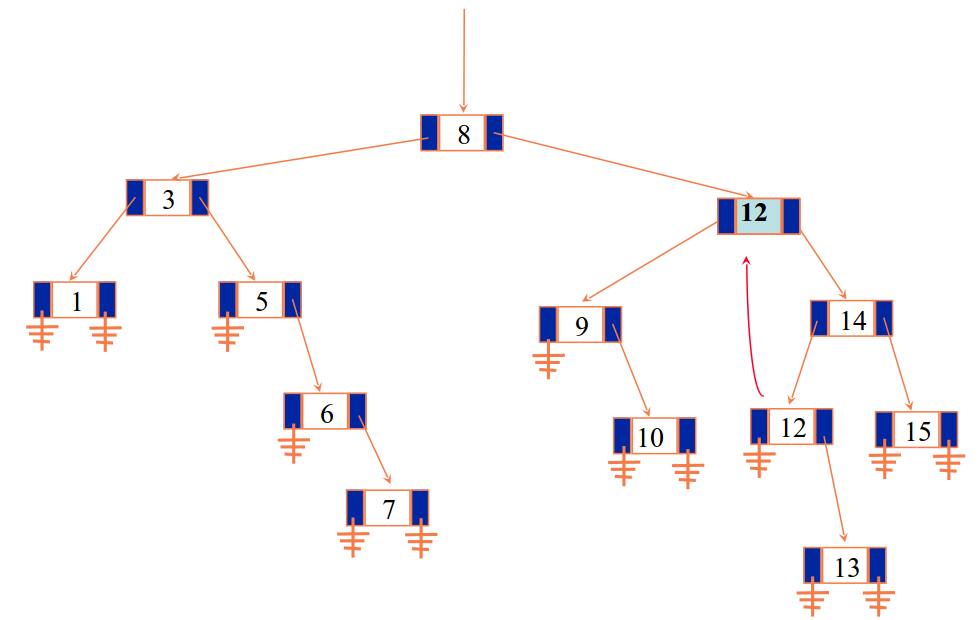
\includegraphics[scale=.3]{arv14.png} 
\end{center}
\end{frame}

\begin{frame}[fragile]{Exemplo}
\setbeamercovered{invisible}
Deleção do nodo com chave = 5
\begin{center}
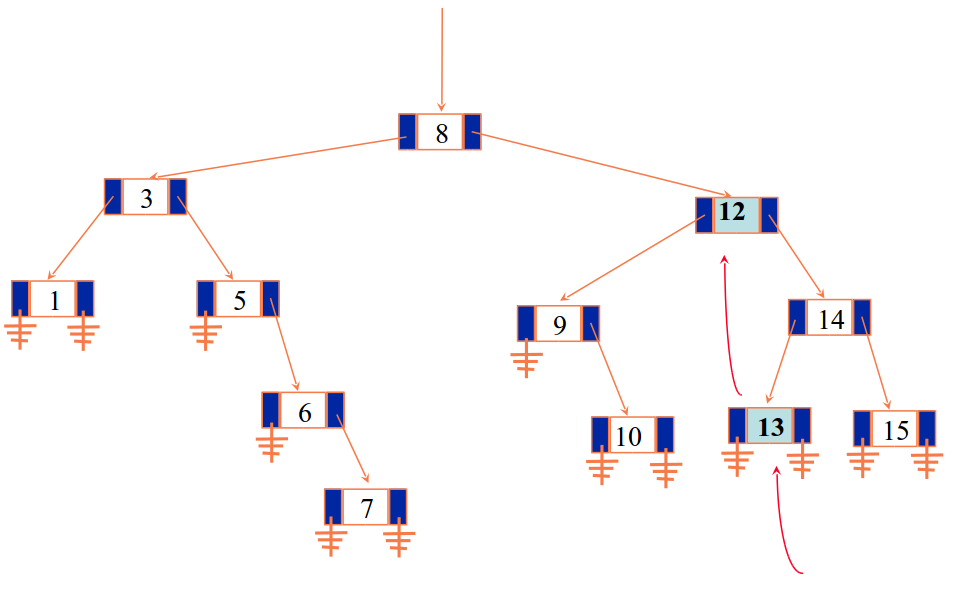
\includegraphics[scale=.3]{arv15.png} 
\end{center}
\end{frame}

\begin{frame}[fragile]{Algoritmo de Deleção}
\lstset{language=C++,
          keywordstyle=\color{blue}\ttfamily,
          stringstyle=\color{red}\ttfamily,
          commentstyle=\color{OliveGreen}\ttfamily,
          breaklines=true,
          basicstyle=\ttfamily\scriptsize
          }
          \begin{lstlisting}
tNodo* delete(info: tInfo, arv: *tNodo)
 tmp, filho: *tNodo;
 início
  se (arv = NULO) então retorne arv
  senão
   se (info < arv->info) // Vá à esquerda.
    arv->filhoÀEsquerda <- delete(info, arv->filhoÀEsquerda);
    retorne arv;
   senão
    se (info > arv->info) // Vá à direita.
     arv->filhoÀDireita <- delete(info, arv->filhoÀDireita);
     retorne arv;
    senão // Encontrei elemento que quero deletar.
     se (arv->filhoÀDireita~=NULO E arv->filhoÀEsquerda~=NULO)//2 filhos.
      tmp <- mínimo(arv->filhoÀDireita); arv->info <- tmp->info;
      arv->filhoÀDireita <-delete(arv->info,arv->filhoÀDireita);
      retorne arv;
      //(CONTINUA NO PROX SLIDE)
		  \end{lstlisting}
\end{frame} 

\begin{frame}[fragile]{Algoritmo de Deleção}
\lstset{language=C++,
          keywordstyle=\color{blue}\ttfamily,
          stringstyle=\color{red}\ttfamily,
          commentstyle=\color{OliveGreen}\ttfamily,
          breaklines=true,
          basicstyle=\ttfamily\scriptsize
          }
          \begin{lstlisting}
     senão // 1 filho.
      tmp <- arv;
      se (arv->filhoÀDireita ~= NULO) então // Filho à direita.
      filho <- arv->filhoÀDireita; retorne filho;
     senão
      se (arv->filhoÀEsquerda ~= NULO) então // Filho à esquerda.
      filho <- arv->filhoÀEsquerda; retorne filho;
     senão // Folha.
      libere arv;
      retorne NULO;
     fim se 
     fim se
     fim se
    fim se 
   fim se
  fim se
 fim
		  \end{lstlisting}
\end{frame} 

\begin{frame}[fragile]{Problemas com Arvores de Busca Binária}
\lstset{language=C++,
          keywordstyle=\color{blue}\ttfamily,
          stringstyle=\color{red}\ttfamily,
          commentstyle=\color{OliveGreen}\ttfamily,
          breaklines=true,
          basicstyle=\ttfamily\footnotesize
          }
          \begin{itemize}
          \item Deterioração:
		  \begin{itemize}
		  \item Quando inserimos utilizando a inserção simples, dependendo da distribuição de dados, pode haver deterioração;
		  \item Árvores deterioradas perdem a característica de eficiência de busca.
		  \end{itemize}
       	  \end{itemize}
\end{frame}

\begin{frame}[fragile]{Problemas com Arvores de Busca Binária}
\setbeamercovered{invisible}
\begin{center}
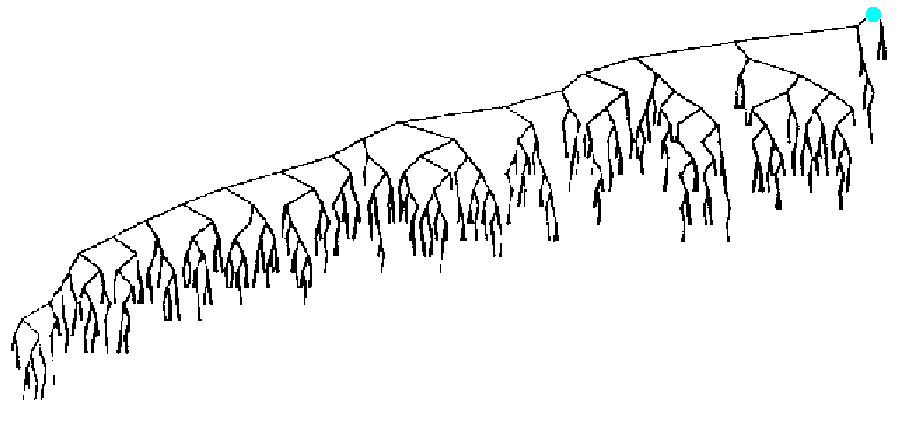
\includegraphics[scale=.35]{deter1.png} 
\end{center}
\end{frame}


\begin{frame}[fragile]{Trabalho}
\lstset{language=C++,
          keywordstyle=\color{blue}\ttfamily,
          stringstyle=\color{red}\ttfamily,
          commentstyle=\color{OliveGreen}\ttfamily,
          breaklines=true,
          basicstyle=\ttfamily\footnotesize
          }
\begin{itemize}
\item Implemente uma classe NoBinario para representar a sua árvore;
\item Implemente a arvore usando Templates;
\item Use as melhores práticas de orientação a objetos;
\item Documente todas as classes, métodos e atributos;
\item Aplique os testes unitários disponíveis no moodle da disciplina para validar sua estrutura de dados;
\item Entregue até a data definida no moodle.
\end{itemize}
\end{frame}

{
\usebackgroundtemplate{
\includegraphics[width=\paperwidth,
height=\paperheight]{../reusable_images/fundo_capa.png}}
\begin{frame}

{\LARGE Perguntas????}

\end{frame}
}


{
\usebackgroundtemplate{
\includegraphics[width=\paperwidth,
height=\paperheight]{../reusable_images/fundo_capa.png}}
\begin{frame}

\includegraphics[scale=0.8]{../reusable_images/cc_logo_arge.png}\hspace{0.5cm}

\includegraphics[scale=0.95]{../reusable_images/by.png}

\vspace{1cm}
Este trabalho está licenciado sob uma Licença Creative Commons Atribuição 4.0 Internacional. Para ver uma cópia desta licença, visite http://creativecommons.org/licenses/by/4.0/.

\end{frame}
}
\end{document}
